\part{Game trees}
\frame{\partpage}

\begin{frame}{State-action graphs}
    \begin{itemize}
        \pause\item We have already discussed \textbf{state-action graphs}
        \begin{itemize}
            \pause\item Nodes: environment states
            \pause\item Edges: actions, which cause transitions from one state to another
        \end{itemize}
        \pause\item Such graphs could contain \textbf{cycles} or \textbf{transpositions}
        \begin{itemize}
            \pause\item Cycle: a sequence of actions which takes us from a state $s_0$ back to the same state $s_0$
            \pause\item Transpositions: two different sequences of actions which both take us from a state $s_1$
                to a state $s_2$
        \end{itemize}
        
    \end{itemize}
\end{frame}

\begin{frame}{State-action trees}
    \begin{itemize}
        \pause\item Searching graphs with cycles and transpositions is tricky
        \pause\item Compare with pathfinding --- needing to store a closed set of already searched nodes
        \pause\item So we often use a \textbf{tree} representation instead
        \pause\item Same state may appear multiple times in the tree
        \pause\item However, there are guaranteed no cycles or transpositions
    \end{itemize}
\end{frame}

\begin{frame}{Example}
	\centering
	\fcolorbox{white}{white}{
		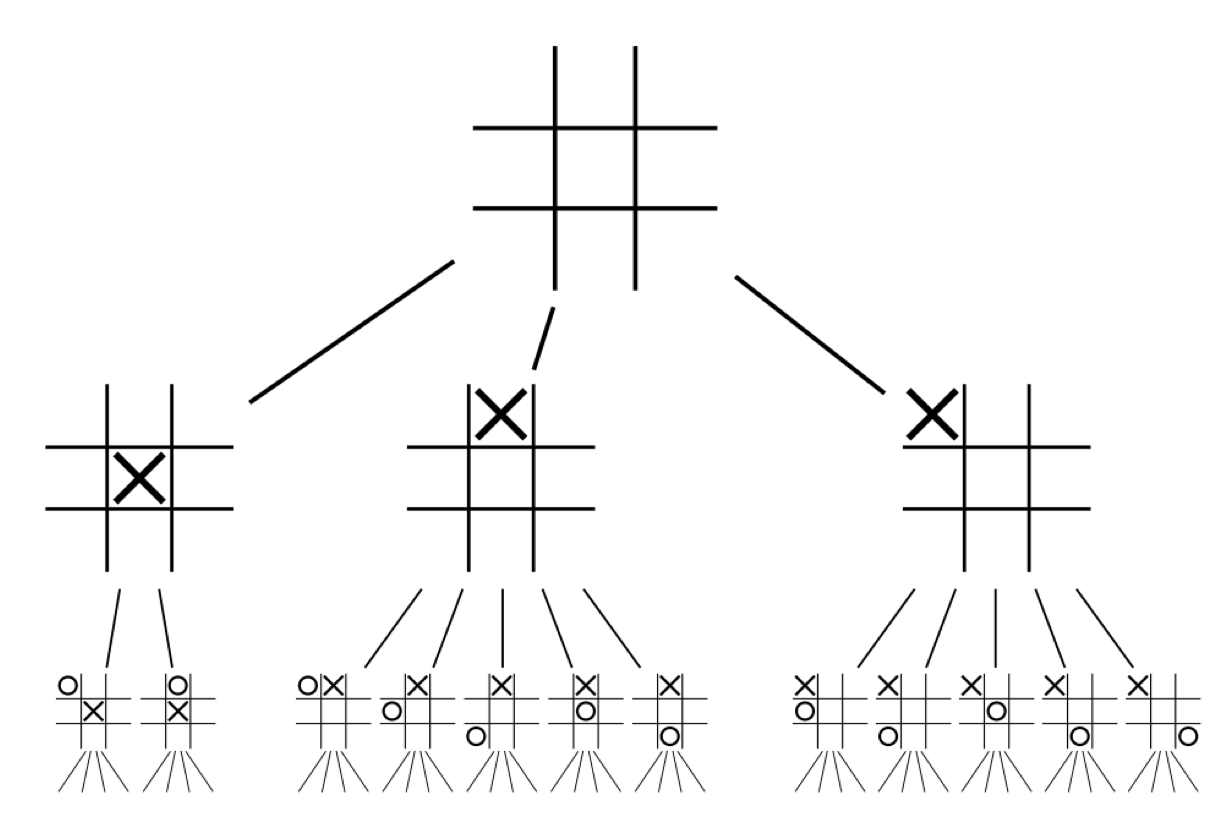
\includegraphics[width=0.8\textwidth]{game_tree}
	}
\end{frame}

